% =====================================================================
% Section 4: CST-Bench (tracks, timing conditions, scorer; <= 1.35 pages
% with Fig. 2 and Table 2). Run-in paragraphs instead of subsections save
% space; the labels sec:bench-taxi, -syn, -timing and -scoring therefore
% resolve to "Section 4" (Secs. 2, 3, 6 and 7 point here).
% Floats: Fig. 2 (figure*, fig:bench) and Table 2 (tables/tab_bench.tex);
% Sec. 5's Fig. 3 (fig:model) is also defined here, before Scoring (placement).
% TAXI numbers are measured on the cstbench v0.1.0 build. Planned: the
% synthetic track, the L1 renders and the scorer parts marked * in Fig. 2.
% Stated once, here: timing-condition parameters, metric equations, the
% CI/bootstrap rule (Sec. 6 relies on it), the TAXI role/language tie and
% the shared-device caveat (Sec. 7 points here).
% Stated elsewhere, not repeated here: the ~200 ms gap and its citations
% (Sec. 1, App. A), routing by language ID (Sec. 1 item (i), Sec. 6.1),
% the release model (Fig. 2 caption, Sec. 1, App. A), the far-field caveat
% (Sec. 7, App. A) and voice consent (App. B, Impact Statement).
% Moved out for space: usable-turn rule, rendering, margins, release and
% caveats -> App. A; Syn sources, Korean MT, voices, TTS editions and QA,
% calibration split, translationese rule -> App. B; normalisation,
% aggregation, detector, metric credits, why StreamLAAL stays primary,
% LongYAAL, the 540-of-554 switch caveat -> App. C; bootstrap and Holm
% details -> App. H.
% Notation: word emission times are t_{n,j}, as t_i in Def. 1 (tau is kept
% for Kendall's statistic); App. C must use the same symbols. Reporting rule as
% stated: Table 3 shows latency next to quality and empty turns; the length
% ratio and the matched-word latency are defined in App. C (both planned).
% =====================================================================
\section{\bench}
\label{sec:bench}\label{sec:bench-design}

\begin{figure*}[t]
  \centering
  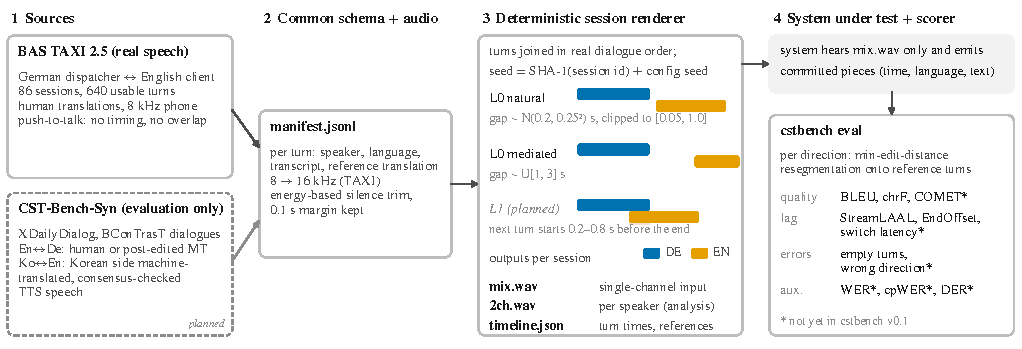
\includegraphics[width=\textwidth]{figures/fig2_benchmark.pdf}
  \caption{The \bench pipeline (planned parts dashed or starred). For TAXI, we release only code, checksums and per-turn scores.}
  \label{fig:bench}
\end{figure*}

\bench renders two-language dialogues as continuous mono sessions that differ only in turn-taking, and scores what a system commits, and when (\cref{fig:bench,tab:bench}). It serves evaluation only; nothing is tuned on \taxi.

% =====================================================================
% Table 2 (tab:bench): CST-Bench composition. Single column; included
% from Sec. 4.2. TAXI L0 values are measured on the cstbench v0.1.0
% build of BAS TAXI 2.5. TAXI L1 and the synthetic track are planned:
% their condition-specific cells use \tbd (plan targets are not facts).
% Measured natural width: 257.9pt at \footnotesize (9pt in ICML), 233.1pt at 8pt (column 234.9pt).
% =====================================================================
\begin{table}[t]
  \caption{\bench composition (TAXI: \taxi; Syn: \syn). TAXI speech, content and turn order are real; its timing is synthetic. The TAXI conditions render the same turns, so merged cells hold for all three. Pairs are \dir{De}{En}\,/\,\dir{En}{De} (German\,/\,English source turns). Speech is counted after silence trimming. Turns/session: median (mean; range); switches: total (median per session). Gaps are taken at speaker changes; occupancy is the share of session time covered by turns. $^\ast$Planned; blank cells are pending. $^\ddagger$English side human, Korean side machine-translated and consensus-checked.}
  \label{tab:bench}
  \centering
  \fontsize{8}{9.5}\selectfont % 8pt (ICML \footnotesize is 9pt): fits the width
  \setlength{\tabcolsep}{3pt}
  \begin{tabular}{@{}lccccc@{}}
    \toprule
    & \multicolumn{3}{c}{TAXI (real speech)} & \multicolumn{2}{c}{Syn (TTS)$^\ast$} \\
    \cmidrule(lr){2-4}\cmidrule(l){5-6}
    & \makecell{L0\\natural} & \makecell{L0\\mediated} & \makecell{L1 turn-end\\overlap$^\ast$} & \pair{En}{De} & \pair{Ko}{En} \\
    \midrule
    Source speech      & \multicolumn{3}{c}{telephone, 8$\to$16\,kHz}     & TTS   & TTS              \\
    References         & \multicolumn{3}{c}{human}                         & human & mixed$^\ddagger$ \\
    Sessions           & \multicolumn{3}{c}{86}                            & \tbd  & \tbd             \\
    Usable turns       & \multicolumn{3}{c}{640 (349\,/\,291)}             & \tbd  & \tbd             \\
    Speech (min)       & \multicolumn{3}{c}{40.378 (17.953\,/\,22.425)}    & \tbd  & \tbd             \\
    Source words       & \multicolumn{3}{c}{6,815 (3,228\,/\,3,587)}       & \tbd  & \tbd             \\
    Reference words    & \multicolumn{3}{c}{6,617 (3,339\,/\,3,278)}       & \tbd  & \tbd             \\
    Mean turn (s)      & \multicolumn{3}{c}{3.086\,/\,4.624}               & \tbd  & \tbd             \\
    Turns/session      & \multicolumn{3}{c}{7 (7.44; 1--17)}               & \tbd  & \tbd             \\
    Switches           & \multicolumn{3}{c}{540 (6)}                       & \tbd  & \tbd             \\
    \midrule
    Session audio (h)  & 0.737  & 0.998  & \tbd & \tbd & \tbd \\
    Median session (s) & 29.023 & 39.316 & \tbd & \tbd & \tbd \\
    Gap mean (s)       & 0.257  & 1.995  & \tbd & \tbd & \tbd \\
    Gap median (s)     & 0.223  & 2.026  & \tbd & \tbd & \tbd \\
    Overlap ratio      & 0.0    & 0.0    & \tbd & \tbd & \tbd \\
    Occupancy (\%)     & 91.27  & 67.42  & \tbd & \tbd & \tbd \\
    \bottomrule
  \end{tabular}
\end{table}


\paragraph{Real track: \taxi.}\label{sec:bench-taxi}
TAXI~2.5 holds telephone dialogues between German-speaking taxi dispatchers and English-speaking clients, with human translations of both sides \citep{bas2001taxi,reichel2016bas}. Push-to-talk recording left one file per turn, without timing or overlap, so in \taxi only the timing is synthetic, and the mono mix of its 640 usable turns simulates a shared device, not the original calls (\cref{app:taxi}). Language coincides with role, and the German dispatcher opens 85 of 86 sessions.

\paragraph{Synthetic track: \syn.}\label{sec:bench-syn}
\draftnote{planned: nothing in this track is built yet}
Voiced by TTS, it cannot replace a real test set but adds overlap measurable at the word level, a distant pair (\pair{Ko}{En}) and both speaker--language assignments, so that language predicts neither role nor first direction. Speakers take turns from two language versions of one XDailyDialog \citep{liu2023xdailydialog} or BConTrasT \citep{farajian2020findings} dialogue, each supplying the other's references; Korean text is consensus-filtered machine translation (\cref{app:syn}).

\paragraph{Timing conditions.}\label{sec:bench-timing}
Turns keep their dialogue order, with within-speaker pauses from $\mathcal{U}[0.3,0.8]$\,s and per-session seeds (\cref{app:taxi}). At speaker changes, \emph{L0 natural} draws gaps from $\mathcal{N}(0.2,0.25^2)$\,s clipped to $[0.05,1]$\,s, around the typical 200\,ms gap, and \emph{L0 mediated} from $\mathcal{U}[1,3]$\,s, as when listeners first read the translation; as gaps separate turn intervals that keep 0.1\,s margins, silences between speech are up to 0.2\,s longer. \emph{L1} starts each new speaker's turn $\mathcal{U}[0.2,0.8]$\,s before the previous one ends, adding overlap to real speech. Per-speaker channels serve an oracle-separation diagnostic.
\draftnote{planned: L1, with a cap for short turns fixed before any baseline run, and word-level overlap; decision needed: whether the L1 overlap is measured between energetic frames or between margin-inclusive intervals, which leaves up to 0.2\,s less overlapping speech}

% Fig. 3 (fig:model) belongs to Sec. 5 but is defined here, so that it floats
% to the top of the page where Sec. 5 starts (a figure* appears at the earliest
% on the page after its definition). Edit its caption here.
\begin{figure*}[t]
  \centering
  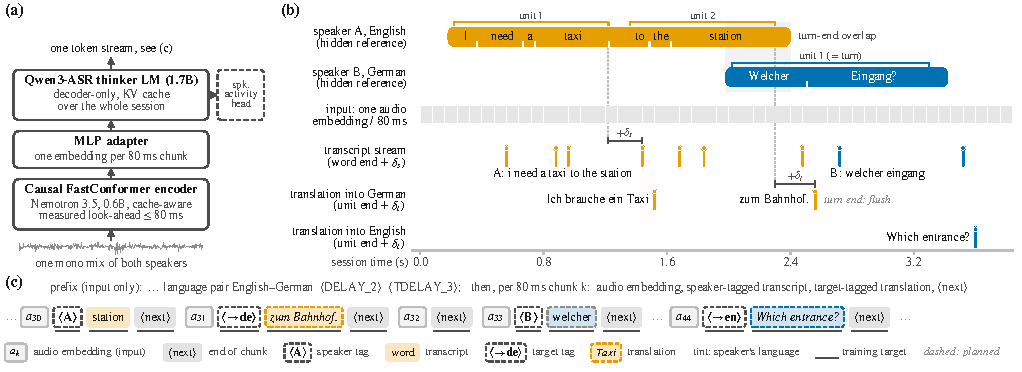
\includegraphics[width=\textwidth]{figures/fig3_model.pdf}
  \caption{\model and conversational delayed streams (illustrative timings; $\delta_s=2$, $\delta_t=3$).
    (a)~Architecture.
    (b)~Targets: a transcript word is due $\delta_s$ chunks, the translation of a verified meaning unit $\delta_t$ chunks, after the chunk in which it ends; a turn end forces a commit.
    (c)~The resulting token stream. Dashed: planned.
    \protect\draftnote{built today: the encoder--adapter--LM backbone, trained for single-speaker English and Korean transcription}}
  \label{fig:model}
\end{figure*}

\paragraph{Scoring.}\label{sec:bench-scoring}
\scorer resegments the committed words of each session and output language onto the references of that direction by word-level Levenshtein alignment \citep{matusov2005evaluating}, keeping each word's emission time, and reports COMET \citep{rei2022comet}, chrF \citep{popovic2015chrf} and BLEU \citep{papineni2002bleu} per direction on lowercased, unpunctuated text (\cref{app:scorer}). For turn $n$, with $L_n=e_n-b_n$ and words $j=1,\dots,|h_n|$ resegmented to it and emitted at $t_{n,j}$, let $d_{n,j}=\max(0,t_{n,j}-b_n)$ and $\rho_n=L_n/\max(|h_n|,|r_n|)$. Then
\begin{align}
  \mathrm{StreamLAAL}_n &= \tfrac{1}{J_n}\textstyle\sum_{j=1}^{J_n}\bigl(d_{n,j}-(j-1)\,\rho_n\bigr), \label{eq:bench-laal}\\
  \mathrm{EndOffset}_n &= t_{n,|h_n|}-e_n, \label{eq:bench-endoffset}\\
  \mathrm{SwitchLatency}_n &= d_{n,1} \quad\text{for } n>1,\ s_n\neq s_{n-1}, \label{eq:bench-switch}
\end{align}
where $J_n$ is the first $j$ with $d_{n,j}\ge L_n$ (else $|h_n|$). \Cref{eq:bench-laal} is length-adaptive Average Lagging (LAAL; \citealp{ma2019stacl,papi2022overgeneration}) on resegmented turns, i.e., \laal \citep{papi2024streamatt}: the lag \emph{within} a turn, $L_n$ for output committed at turn ends. As \laal ignores words after $J_n$, \eo, SimulEval's EndOffset taken per turn \citep{ma2020simuleval,seamless2023seamless}, measures the wait after the speaker stops; switch latency is the matching StartOffset at direction changes. A committed piece is \emph{wrong-direction} if turns are open but none is translated into its language, if a text language identifier assigns it to the other language, or if it copies an open turn's transcript; we report the share of committed words in such pieces. Transcripts are scored by WER and cpWER (\citealp{watanabe2020chime}; for Korean, cpCER on characters), speakers by DER.

\paragraph{Statistics and validation.}
Comparisons carry 95\% confidence intervals (CIs) from a session-clustered paired bootstrap \citep{koehn2004statistical}; main comparisons, fixed before the test runs, are Holm-corrected (\citealp{holm1979simple}; \cref{app:repro}). Controlled perturbations of the reference output test whether BLEU, chrF, \laal, \eo and wrong-direction words move only as expected (\cref{tab:sanity}). Copying the source lowered \deen \laal below that of the reference committed at turn ends (\prelim{2.276} vs.\ \prelim{3.086}\,s; $^\dagger$preliminary), so \cref{tab:main} shows latency next to quality and empty turns, and \cref{app:scorer} defines a matched-word latency.
\draftnote{scorer v0.1 computes BLEU, chrF, \laal, \eo, empty turns and wrong-language words given gold turn IDs; the other metrics (including the length ratio and the matched-word latency), the bootstrap and a pinned number normaliser are being added; rows 3--10 of \cref{tab:sanity} are planned}
